\chapter{Probabilidade, amostragem e estimação}
\label{cap:probabilidade}

Nos capítulos anteriores, usamos médias, erros padrão, valores de $p$ e intervalos de confiança. Vamos agora olhar com mais cuidado para as ideias que sustentam esses cálculos. O objetivo é conseguir explicar o que varia entre pessoas, o que varia entre amostras e o que um modelo de probabilidade acrescenta à análise.

Você pode estudar este capítulo antes dos testes de hipóteses ou retomá-lo como uma revisão. Vamos partir de exemplos pequenos, desenhar as situações e só então escrever as fórmulas. Ao final, faremos uma primeira experiência de reamostragem no Rj.

\section{Eventos, probabilidades e denominadores}

Uma probabilidade descreve a possibilidade de um evento dentro de um modelo. Se representamos por $A$ o evento de interesse, escrevemos $P(A)$, com $0\leq P(A)\leq1$. O evento complementar, $A^c$, reúne os resultados que não pertencem a $A$:
\[
P(A^c)=1-P(A).
\]
Uma probabilidade de $0{,}30$ corresponde a 30\%, mas não significa que em cada dez observações ocorrerão exatamente três resultados do evento. Repetições podem produzir contagens diferentes.

Na tabela do capítulo~\ref{cap:categoricos}, os grupos A e B têm 50 pessoas cada. O resultado Sim aparece em 45 das 100 observações. Defina $G$ como pertencer ao grupo A e $S$ como apresentar Sim. Assim, $P(G)=0{,}50$ e a frequência relativa de Sim no banco é $45/100=0{,}45$. Nesta discussão, vamos usar a distribuição empírica do arquivo como modelo ilustrativo.

\subsection{Probabilidade conjunta e condicional}

O evento $G\cap S$ exige duas condições ao mesmo tempo: pertencer ao grupo A e apresentar Sim. Há 30 observações nessa célula, portanto $P(G\cap S)=30/100=0{,}30$. Já a probabilidade condicional restringe o denominador ao grupo informado:
\[
P(S\mid G)=\frac{P(S\cap G)}{P(G)}
=\frac{0{,}30}{0{,}50}=0{,}60.
\]
O símbolo $\mid$ pode ser lido como ``dado que''. Estamos perguntando a frequência de Sim entre as pessoas do grupo A. Se invertermos a condição, teremos outra pergunta:
\[
P(G\mid S)=\frac{30}{45}\approx0{,}667.
\]
Agora o denominador contém somente as pessoas que apresentaram Sim. As duas quantidades não precisam ser iguais.

\begin{figure}[H]
\centering
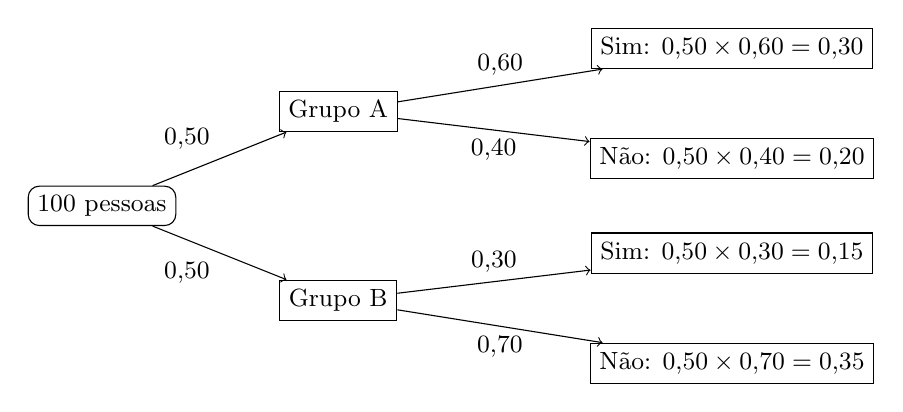
\begin{tikzpicture}[x=1cm,y=1cm,every node/.style={font=\small}]
  \node[draw,rounded corners,align=center] (origem) at (0,0) {100 pessoas};
  \node[draw] (ga) at (3,1.2) {Grupo A};
  \node[draw] (gb) at (3,-1.2) {Grupo B};
  \node[draw,align=left] (as) at (8,2) {Sim: $0{,}50\times0{,}60=0{,}30$};
  \node[draw,align=left] (an) at (8,0.6) {Não: $0{,}50\times0{,}40=0{,}20$};
  \node[draw,align=left] (bs) at (8,-0.6) {Sim: $0{,}50\times0{,}30=0{,}15$};
  \node[draw,align=left] (bn) at (8,-2) {Não: $0{,}50\times0{,}70=0{,}35$};
  \draw[->] (origem) -- node[above left] {$0{,}50$} (ga);
  \draw[->] (origem) -- node[below left] {$0{,}50$} (gb);
  \draw[->] (ga) -- node[above] {$0{,}60$} (as);
  \draw[->] (ga) -- node[below] {$0{,}40$} (an);
  \draw[->] (gb) -- node[above] {$0{,}30$} (bs);
  \draw[->] (gb) -- node[below] {$0{,}70$} (bn);
\end{tikzpicture}
\caption{Árvore das proporções da tabela fictícia. O produto ao longo de cada caminho fornece uma probabilidade conjunta; as quatro folhas somam 1. Elaboração própria.}
\label{fig:arvore-probabilidades}
\end{figure}

A regra do produto permite escrever $P(G\cap S)=P(G)P(S\mid G)$. Somando as duas maneiras de chegar a Sim, obtemos:
\[
P(S)=P(G)P(S\mid G)+P(G^c)P(S\mid G^c)
=0{,}30+0{,}15=0{,}45.
\]
Da mesma decomposição vem a regra de Bayes:
\[
P(G\mid S)=\frac{P(S\mid G)P(G)}{P(S)}.
\]
Ela reorganiza probabilidades condicionais; não transforma uma associação em explicação causal. Sempre identifique quais eventos foram condicionados e qual população o modelo descreve.

\subsection{Independência}

Dois eventos são independentes quando $P(A\cap B)=P(A)P(B)$. Se $P(B)>0$, isso equivale a $P(A\mid B)=P(A)$. No nosso exemplo, $P(S\mid G)=0{,}60$ difere de $P(S)=0{,}45$: na distribuição empírica, as variáveis estão associadas.

Esse uso da palavra independência se refere à relação entre eventos ou variáveis. Já a independência das \textbf{observações} diz respeito à estrutura das unidades do estudo. Uma tabela pode mostrar associação entre grupo e resultado e, ainda assim, ter pessoas independentes entre si. São perguntas diferentes, ambas relevantes para a análise.

\section{Da observação à variável aleatória}

Uma variável aleatória associa números aos resultados de um processo. Antes de observar quatro respostas, por exemplo, o total de respostas Sim ainda pode ser 0, 1, 2, 3 ou 4. Depois da coleta, observaremos um desses valores.

Para uma variável discreta $X$, a função de probabilidade atribui uma massa $P(X=x)$ a cada valor possível. A soma de todas as massas precisa ser 1. A esperança é uma média ponderada pelas probabilidades:
\[
E(X)=\sum_x xP(X=x),\qquad
\operatorname{Var}(X)=\sum_x\{x-E(X)\}^2P(X=x).
\]
A esperança não precisa ser um resultado possível de uma única observação. Um número esperado de $2{,}4$ respostas Sim não implica a existência de uma pessoa fracionada.

Para uma variável contínua, usamos uma densidade $f(x)$. A probabilidade de um intervalo é uma área:
\[
P(a\leq X\leq b)=\int_a^b f(x)\,dx.
\]
A altura da curva em um ponto não é a probabilidade desse ponto. No modelo contínuo, $P(X=x)=0$ para um valor isolado, embora intervalos tenham probabilidades positivas. Medidas registradas com arredondamento representam faixas de valores do processo de medição.

\section{Modelo binomial: contando resultados}

Considere quatro observações independentes, cada uma com probabilidade $\pi=0{,}60$ de Sim. Se $X$ conta quantas respostas Sim ocorreram, então $X\sim\operatorname{Binomial}(n=4,\pi=0{,}60)$. A distribuição supõe o mesmo valor de $\pi$ para as quatro observações.

A probabilidade de exatamente $k$ resultados Sim é:
\[
P(X=k)=\binom{n}{k}\pi^k(1-\pi)^{n-k},
\qquad \binom{n}{k}=\frac{n!}{k!(n-k)!}.
\]
A potência $\pi^k(1-\pi)^{n-k}$ corresponde à probabilidade de uma sequência particular. O coeficiente binomial conta quantas sequências diferentes têm a mesma quantidade de resultados Sim. O NIST apresenta essa definição e os parâmetros do modelo \parencite{NISTBinomial}.

Para exatamente três resultados Sim, há quatro posições possíveis para o único Não. Logo,
\[
P(X=3)=4\times0{,}60^3\times0{,}40=0{,}3456.
\]
Para pelo menos três, somamos $P(X=3)+P(X=4)=0{,}3456+0{,}1296=0{,}4752$. ``Exatamente três'' e ``pelo menos três'' delimitam eventos diferentes.

\begin{figure}[H]
\centering
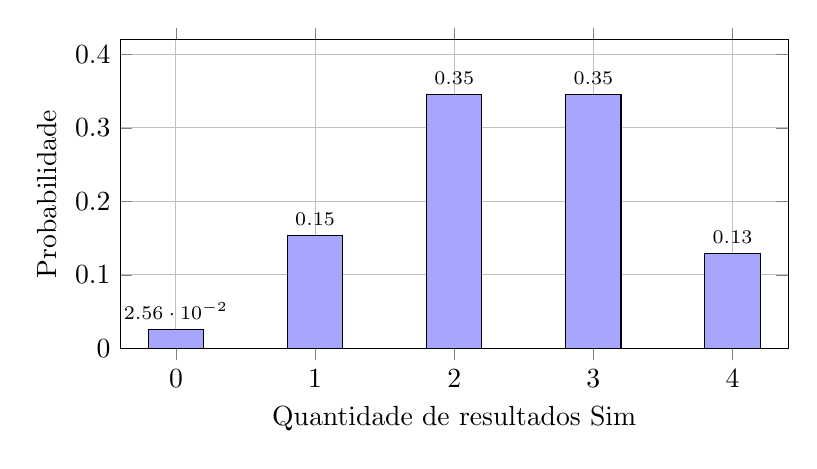
\begin{tikzpicture}
\begin{axis}[
  ybar,width=0.83\textwidth,height=5.5cm,
  xlabel={Quantidade de resultados Sim},ylabel={Probabilidade},
  xtick={0,1,2,3,4},ymin=0,ymax=0.42,
  bar width=20pt,nodes near coords,
  every node near coord/.append style={font=\scriptsize},
  grid=major
]
  \addplot[fill=blue!35] coordinates
    {(0,0.0256) (1,0.1536) (2,0.3456) (3,0.3456) (4,0.1296)};
\end{axis}
\end{tikzpicture}
\caption{Distribuição binomial para quatro observações e probabilidade de Sim igual a 0,60. As barras somam 1. Elaboração própria.}
\label{fig:binomial-quatro}
\end{figure}

Nesse modelo, $E(X)=n\pi=2{,}4$ e $\operatorname{Var}(X)=n\pi(1-\pi)=0{,}96$. No Rj, a instrução \texttt{dbinom(3, size = 4, prob = 0.6)} calcula a probabilidade exata de três, enquanto \texttt{pbinom(2, 4, 0.6, lower.tail = FALSE)} calcula a de mais de dois. A documentação oficial do R distingue a massa pontual, a probabilidade acumulada, os quantis e a geração aleatória \parencite{RDistribuicaoBinomial}.

\section{Distribuição normal e padronização}

O modelo normal é contínuo, simétrico e definido pela média $\mu$ e pelo desvio padrão $\sigma>0$. Escrevemos $X\sim N(\mu,\sigma^2)$; o segundo parâmetro nessa notação é a \textbf{variância}. Sua densidade é:
\[
f(x)=\frac{1}{\sigma\sqrt{2\pi}}
\exp\left\{-\frac{(x-\mu)^2}{2\sigma^2}\right\}.
\]
A padronização $Z=(X-\mu)/\sigma$ leva à normal padrão, com média 0 e variância 1. A documentação oficial do R permite calcular suas áreas com \texttt{pnorm} e seus quantis com \texttt{qnorm} \parencite{RNormal}.

Suponha, como modelo ilustrativo, $X\sim N(60,10^2)$. Uma nota 70 fica um desvio padrão acima da média: $z=(70-60)/10=1$. A probabilidade de uma nota entre 50 e 70 é $P(-1\leq Z\leq1)\approx0{,}683$. Para a faixa entre 40 e 80, são dois desvios padrão para cada lado, com probabilidade aproximada de $0{,}954$.

\begin{figure}[H]
\centering
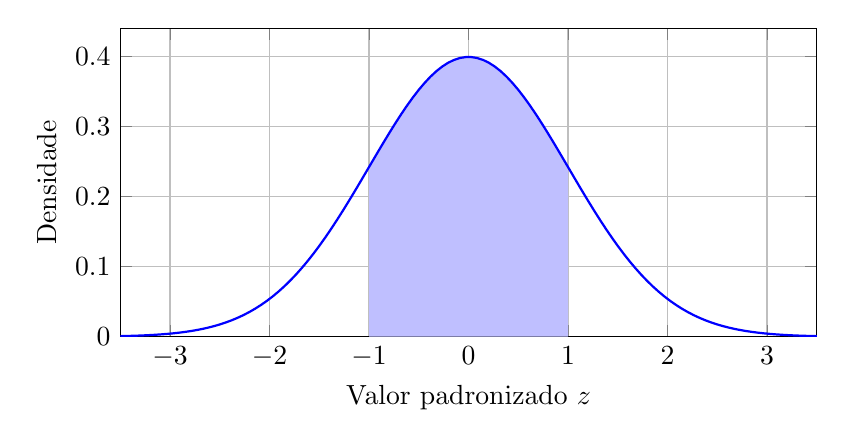
\begin{tikzpicture}
\begin{axis}[
  width=0.86\textwidth,height=5.5cm,
  xlabel={Valor padronizado $z$},ylabel={Densidade},
  xmin=-3.5,xmax=3.5,ymin=0,ymax=0.44,
  xtick={-3,-2,-1,0,1,2,3},grid=major
]
  \addplot[draw=none,fill=blue!25,domain=-1:1,samples=70]
    {exp(-x*x/2)/sqrt(2*pi)} \closedcycle;
  \addplot[blue,thick,domain=-3.5:3.5,samples=120]
    {exp(-x*x/2)/sqrt(2*pi)};
\end{axis}
\end{tikzpicture}
\caption{Na normal padrão, a área entre $-1$ e 1 é aproximadamente 68,3\%. A altura da curva é densidade, não probabilidade pontual. Elaboração própria.}
\label{fig:normal-area}
\end{figure}

Essas porcentagens pertencem ao modelo normal. Não devem ser aplicadas a toda variável apenas porque conhecemos sua média e seu desvio padrão. Notas têm limites substantivos, podem apresentar concentração nos extremos e não precisam seguir exatamente essa distribuição. Examine os dados e o papel da suposição no procedimento escolhido.

\section{Pessoas variam; médias amostrais também}
\label{sec:distribuicao-amostral}

Imagine repetir um processo de amostragem e calcular uma média em cada amostra. A distribuição dessas médias é a \textbf{distribuição amostral da média}. Ela é diferente da distribuição das observações individuais que compõem cada amostra.

Para observações independentes, com mesma média $\mu$ e variância finita $\sigma^2$, temos:
\[
E(\bar{X})=\mu,\qquad
\operatorname{Var}(\bar{X})=\frac{\sigma^2}{n},\qquad
DP(\bar{X})=\frac{\sigma}{\sqrt{n}}.
\]
O último termo é o erro padrão populacional da média. Na prática, quando $\sigma$ é desconhecido, usamos $s/\sqrt{n}$ como estimativa, sob as condições correspondentes.

\begin{figure}[H]
\centering
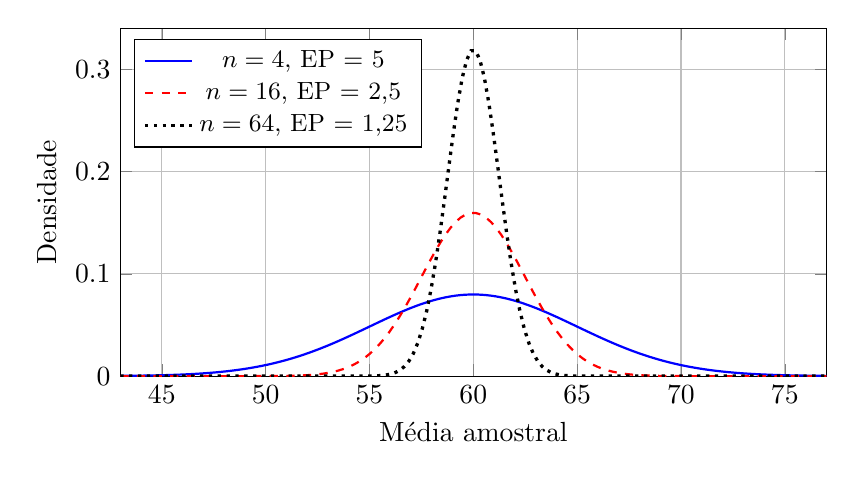
\begin{tikzpicture}
\begin{axis}[
  width=0.87\textwidth,height=6cm,
  xlabel={Média amostral},ylabel={Densidade},
  xmin=43,xmax=77,ymin=0,ymax=0.34,grid=major,
  legend style={at={(0.02,0.97)},anchor=north west,font=\small}
]
  \addplot[blue,thick,domain=43:77,samples=140]
    {exp(-((x-60)/5)^2/2)/(5*sqrt(2*pi))};
  \addlegendentry{$n=4$, EP = 5}
  \addplot[red,dashed,thick,domain=43:77,samples=140]
    {exp(-((x-60)/2.5)^2/2)/(2.5*sqrt(2*pi))};
  \addlegendentry{$n=16$, EP = 2,5}
  \addplot[black,dotted,very thick,domain=43:77,samples=160]
    {exp(-((x-60)/1.25)^2/2)/(1.25*sqrt(2*pi))};
  \addlegendentry{$n=64$, EP = 1,25}
\end{axis}
\end{tikzpicture}
\caption{Distribuições exatas da média para amostras independentes de uma população normal com $\mu=60$ e $\sigma=10$. Aumentar $n$ reduz a dispersão das médias; o DP das pessoas continua igual a 10. Elaboração própria.}
\label{fig:medias-amostrais}
\end{figure}

O teorema central do limite explica por que a normal também aparece como aproximação da distribuição de médias quando a população não é normal. Na versão clássica para observações independentes e identicamente distribuídas, com variância finita e positiva, a média padronizada aproxima-se da normal conforme $n$ cresce \parencite{NISTNormal}.

Isso não estabelece uma regra universal de que ``30 observações resolvem a normalidade''. Assimetria intensa, caudas pesadas e observações influentes podem dificultar a aproximação em tamanhos usuais. Dependência entre registros também exige outro tratamento. O teorema fala da distribuição do estimador sob condições, e não de uma transformação automática dos dados individuais em uma curva normal.

\subsection{Precisão e viés são questões diferentes}

Quadruplicar $n$, mantendo as demais condições, reduz o erro padrão pela metade. Para passar de EP 5 a EP 2,5, precisamos aumentar a amostra de 4 para 16, como na figura~\ref{fig:medias-amostrais}. O ganho segue a raiz quadrada, não uma relação diretamente proporcional ao número de observações.

Uma amostra maior, porém, não corrige necessariamente seleção inadequada. Se convidamos apenas pessoas muito interessadas no tema para estimar o comportamento de toda a população, podemos obter uma estimativa precisa para um grupo que não representa nosso alvo. Precisão descreve a dispersão do estimador; viés descreve seu afastamento sistemático em relação ao parâmetro sob o processo de amostragem.

\begin{figure}[H]
\centering
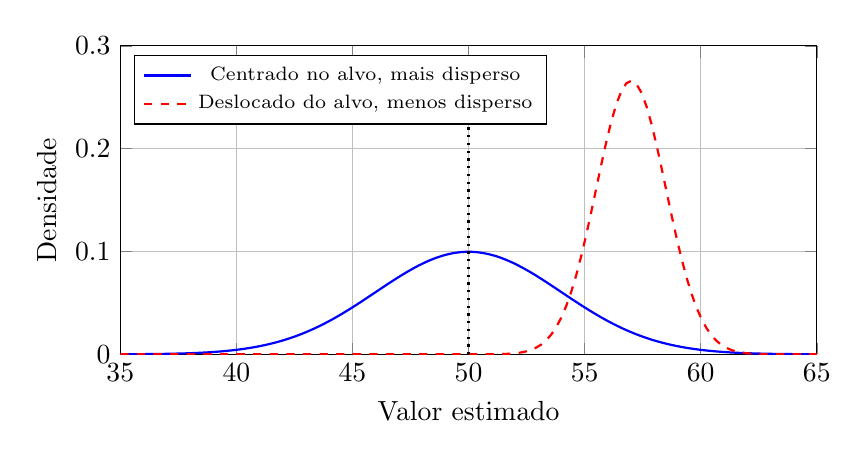
\begin{tikzpicture}
\begin{axis}[
  width=0.86\textwidth,height=5.5cm,
  xlabel={Valor estimado},ylabel={Densidade},
  xmin=35,xmax=65,ymin=0,ymax=0.30,grid=major,
  legend style={at={(0.02,0.97)},anchor=north west,font=\scriptsize}
]
  \addplot[blue,thick,domain=35:65,samples=120]
    {exp(-((x-50)/4)^2/2)/(4*sqrt(2*pi))};
  \addlegendentry{Centrado no alvo, mais disperso}
  \addplot[red,dashed,thick,domain=35:65,samples=140]
    {exp(-((x-57)/1.5)^2/2)/(1.5*sqrt(2*pi))};
  \addlegendentry{Deslocado do alvo, menos disperso}
  \addplot[black,dotted,thick] coordinates {(50,0) (50,0.29)};
\end{axis}
\end{tikzpicture}
\caption{Precisão e viés em distribuições esquemáticas de estimadores. A linha vertical marca o parâmetro 50. Uma distribuição estreita pode estar afastada do alvo. Elaboração própria.}
\label{fig:vies-precisao}
\end{figure}

Antes de calcular o tamanho de uma amostra, defina quem está na população de interesse, como cada unidade pode ser selecionada e o que ocorre com as não respostas. Uma grande quantidade de linhas não substitui esse planejamento.

\section{Intervalos de confiança: a lógica das repetições}

Um intervalo usual para uma média, com desvio padrão populacional desconhecido e condições adequadas para a inferência t, é:
\[
\bar{x}\ \pm\ t_{1-\alpha/2,n-1}\frac{s}{\sqrt{n}}.
\]
A estimativa está no centro, o quantil estabelece o nível do procedimento e o erro padrão informa a precisão. O NIST apresenta essa construção para a média \parencite{NISTIntervalo}. A distribuição t considera a estimação da variabilidade; com poucos graus de liberdade, seus quantis de cauda são maiores que os da normal padrão \parencite{RTStudent}.

Por exemplo, o quantil bilateral de 95\% é aproximadamente 2,571 com cinco graus de liberdade, 2,110 com 17 e 1,960 no limite normal. Não basta trocar todos por 1,96 em qualquer amostra. No arquivo de notas, o IC95\% da média posterior usa 17 graus de liberdade e foi apresentado no capítulo~\ref{cap:hipoteses}.

\begin{figure}[H]
\centering
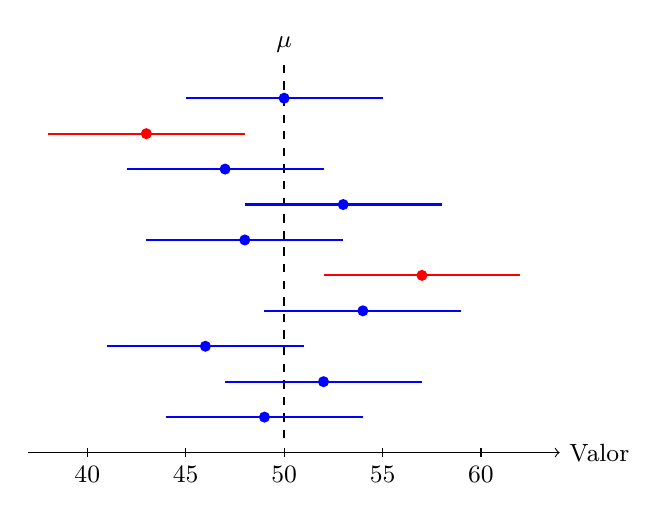
\begin{tikzpicture}[x=0.25cm,y=0.45cm,every node/.style={font=\small}]
  \draw[->] (37,0) -- (64,0) node[right] {Valor};
  \foreach \x in {40,45,50,55,60} {
    \draw (\x,0.13) -- (\x,-0.13) node[below] {\x};
  }
  \draw[dashed,thick] (50,0.4) -- (50,11) node[above] {$\mu$};
  \foreach \y/\a/\b/\m in {1/44/54/49,2/47/57/52,3/41/51/46,4/49/59/54,6/43/53/48,7/48/58/53,8/42/52/47,10/45/55/50} {
    \draw[blue,thick] (\a,\y) -- (\b,\y);
    \fill[blue] (\m,\y) circle (2pt);
  }
  \foreach \y/\a/\b/\m in {5/52/62/57,9/38/48/43} {
    \draw[red,thick] (\a,\y) -- (\b,\y);
    \fill[red] (\m,\y) circle (2pt);
  }
\end{tikzpicture}
\caption{Intervalos esquemáticos de diferentes amostras. Em vermelho estão os que não incluem o parâmetro fixo. O desenho ilustra a lógica de cobertura; sua contagem não é uma estimativa da cobertura de um procedimento. Elaboração própria.}
\label{fig:cobertura-intervalos}
\end{figure}

Na interpretação frequentista, o parâmetro é fixo e os limites mudam entre amostras. Um procedimento de 95\% de confiança cobre o parâmetro em 95\% das repetições, sob suas condições. Isso não obriga exatamente 19 de cada 20 intervalos consecutivos a cobrir o parâmetro, nem transforma o intervalo observado em uma região que contém 95\% das pessoas.

Aumentar o nível de confiança, mantendo os mesmos dados e método, alarga o intervalo. Aumentar o tamanho amostral tende a estreitá-lo, mantidas as demais condições. Essas escolhas devem ser ligadas à pergunta: precisamos distinguir uma faixa pequena de valores ou basta uma estimativa inicial com incerteza maior?

\section{Bootstrap: reamostrando os dados observados}

Outra forma de estudar a variabilidade de um estimador é reamostrar as observações. No bootstrap não paramétrico simples para unidades independentes, sorteamos $n$ registros \textbf{com reposição} da amostra original de tamanho $n$ e recalculamos a estatística. Repetimos o processo muitas vezes.

Com reposição significa que uma observação pode aparecer várias vezes em uma reamostra e outra pode não aparecer. Não estamos coletando participantes novos: usamos a distribuição empírica para aproximar a variabilidade do estimador. O pacote oficial \texttt{boot} do R documenta diferentes esquemas de reamostragem \parencite{RBootstrap}.

\begin{figure}[H]
\centering
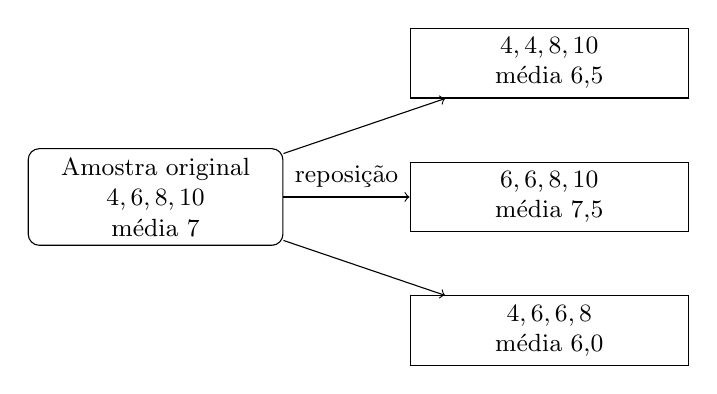
\begin{tikzpicture}[x=1cm,y=1cm,every node/.style={font=\small}]
  \node[draw,rounded corners,align=center,text width=3cm] (dados) at (0,0)
    {Amostra original\\$4,6,8,10$\\média $7$};
  \node[draw,align=center,text width=3.3cm] (b1) at (5,1.7)
    {$4,4,8,10$\\média $6{,}5$};
  \node[draw,align=center,text width=3.3cm] (b2) at (5,0)
    {$6,6,8,10$\\média $7{,}5$};
  \node[draw,align=center,text width=3.3cm] (b3) at (5,-1.7)
    {$4,6,6,8$\\média $6{,}0$};
  \draw[->] (dados) -- (b1);
  \draw[->] (dados) -- node[above] {reposição} (b2);
  \draw[->] (dados) -- (b3);
\end{tikzpicture}
\caption{Três reamostras possíveis de um conjunto pequeno. São apenas uma ilustração do mecanismo; três reamostras não bastam para construir um intervalo útil. Elaboração própria.}
\label{fig:bootstrap-mecanismo}
\end{figure}

\subsection{Uma experiência no Rj}

Abra \texttt{exemplo\_notas.csv} e, no Rj, use o banco disponível como \texttt{data}. O código abaixo calcula 5.000 médias de reamostras da nota posterior:

\begin{verbatim}
set.seed(20261025)
x <- data$depois
x <- x[!is.na(x)]
medias <- replicate(5000, {
    indices <- sample.int(length(x), size = length(x),
                          replace = TRUE)
    mean(x[indices])
})
mean(x)
sd(medias)
quantile(medias, c(0.025, 0.975))
\end{verbatim}

A semente permite repetir o experimento no mesmo ambiente. A documentação de \texttt{sample} descreve o sorteio com reposição e a função \texttt{sample.int} usada para selecionar índices \parencite{RAmostragem}. O desvio padrão das médias reamostradas estima a variabilidade do estimador; os quantis delimitam um intervalo percentil ilustrativo. Ele não precisa coincidir com o intervalo t.

Aumentar o número de reamostras reduz a variação de Monte Carlo do cálculo, mas não aumenta a amostra de pessoas. Além disso, o bootstrap simples não corrige seleção inadequada nem serve indistintamente para dependência, séries temporais ou conglomerados. Para um antes/depois, reamostre a pessoa com seu par completo, ou a diferença individual quando ela for a unidade da análise. Sortear as duas colunas separadamente destruiria a estrutura do problema.

\section{Vamos praticar: perguntas e comentários}

\begin{enumerate}
  \item Na tabela fictícia, por que $P(S\mid G)=30/50$ difere de $P(G\mid S)=30/45$?
  \item No modelo binomial de quatro observações, calcule a probabilidade de pelo menos três respostas Sim.
  \item Se o DP populacional permanece 10, qual é o EP da média com $n=25$ e com $n=100$?
  \item Uma amostra maior corrige necessariamente o viés de seleção?
  \item Um IC95\% da média contém 95\% das notas individuais?
  \item Ao passar de 5.000 para 20.000 reamostras bootstrap, quadruplicamos o número de participantes?
\end{enumerate}

\subsection*{Comentários das respostas}

\begin{enumerate}
  \item As condições alteram os conjuntos de referência: a primeira restringe ao grupo A; a segunda, às respostas Sim.
  \item $0{,}3456+0{,}1296=0{,}4752$, somando os eventos $X=3$ e $X=4$.
  \item $10/\sqrt{25}=2$ e $10/\sqrt{100}=1$, sob as condições da fórmula.
  \item Não. Uma estimativa pode ficar menos dispersa e continuar sistematicamente afastada da população de interesse.
  \item Não. Ele expressa a incerteza do procedimento de estimação da média; a distribuição das pessoas é outra questão.
  \item Não. Continuamos usando as mesmas pessoas, com mais repetições do algoritmo de reamostragem.
\end{enumerate}
